\documentclass[../main.tex]{subfiles}
\begin{document}

Character detection done by our LSVC is shown in \autoref{fig:detection_small} and
\autoref{fig:detection_large}. The character detection system performs really
well on the test image, but not so great on the larger one. There might be
several reasons to this. The authors argue that the cleanliness of
\autoref{fig:detection_small} helps the system to only classify pictures of
characters as actual characters. However, confusion arise when the sliding
window is focused on more than one character at a time. Such an outcrop of two
characters is completely new to the classifier, and the outcrop is misclassified.

The character detection system can be improved by adding additional image
processing before character classification. The additional processing would help
misclassifying white images as the character `i'. The authors would also look
into adding white images with class `background' in the dataset. Our classifier
would then train to distinguish between characters and background.


\begin{figure}[t!]
  \hspace{3.9cm}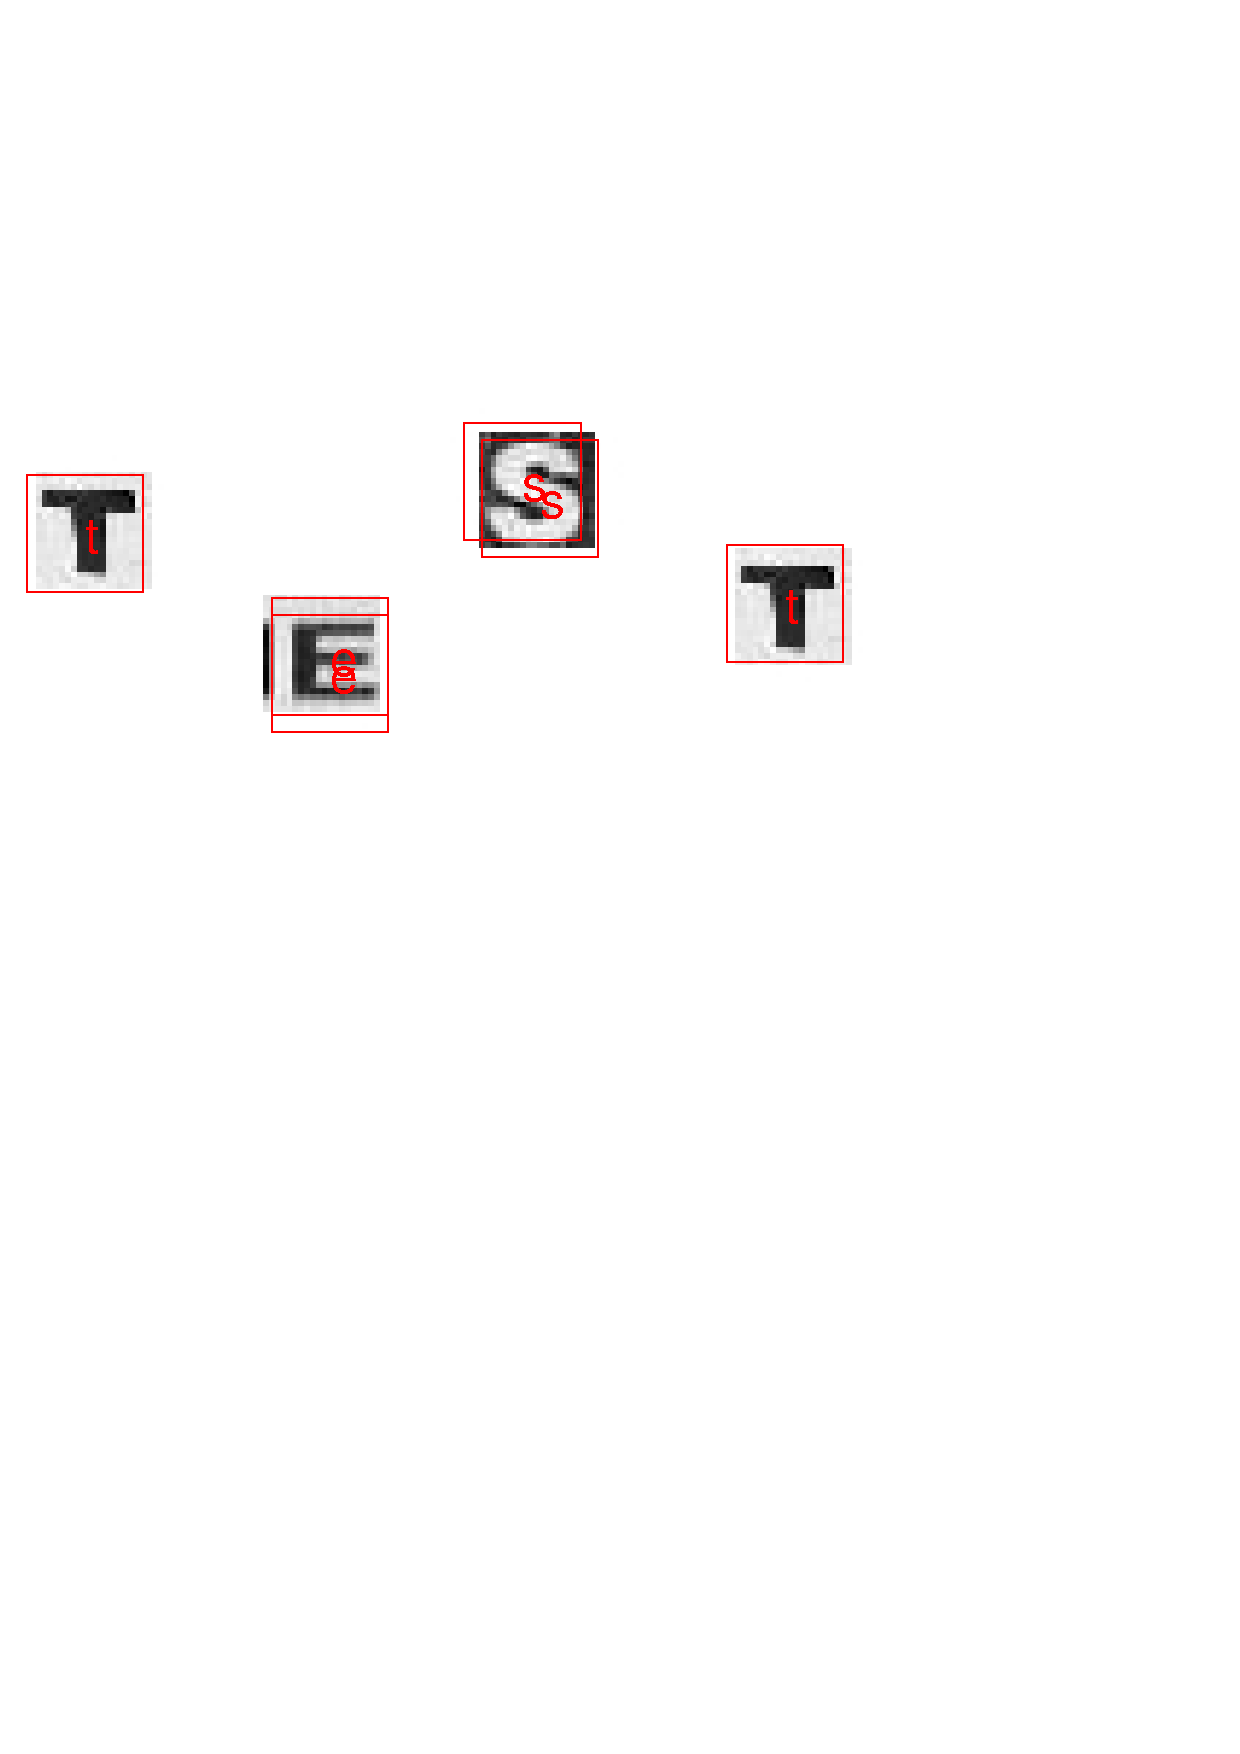
\includegraphics[trim={4cm, 15cm, 4cm, 1cm},width=0.5\textwidth]{figures/character_detection/detection_2.pdf}
  \caption{Detection on test image.}
  \label{fig:detection_small}
\end{figure}

\begin{figure}
  \hspace*{2.4cm}
\includegraphics[trim={4cm, 12cm, 4cm, 10cm},width=0.7\textwidth]{figures/character_detection/detection_1.pdf}
  \caption{Detection on a larger image.}
  \label{fig:detection_large}
\end{figure}
\end{document}